\chapter{Introduction} %\label{ch:intro}

\section{Zero Point Energy and the Dynamical Casimir Effect}\label{sec:ZPE_and_DCE}
\section{Superconducting circuits and SQUIDS}\label{sec:SC_and_SQUIDs}
\section{DCE in Superconducting Circuits}\label{sec:DCE_in_SC}
\section{Kronig-Penney Model in Solid State Physics}\label{sec:KP_in_SS}
 %\cite{Garza:2011fk}

\begin{comment}
\begin{figure}
  \centering
  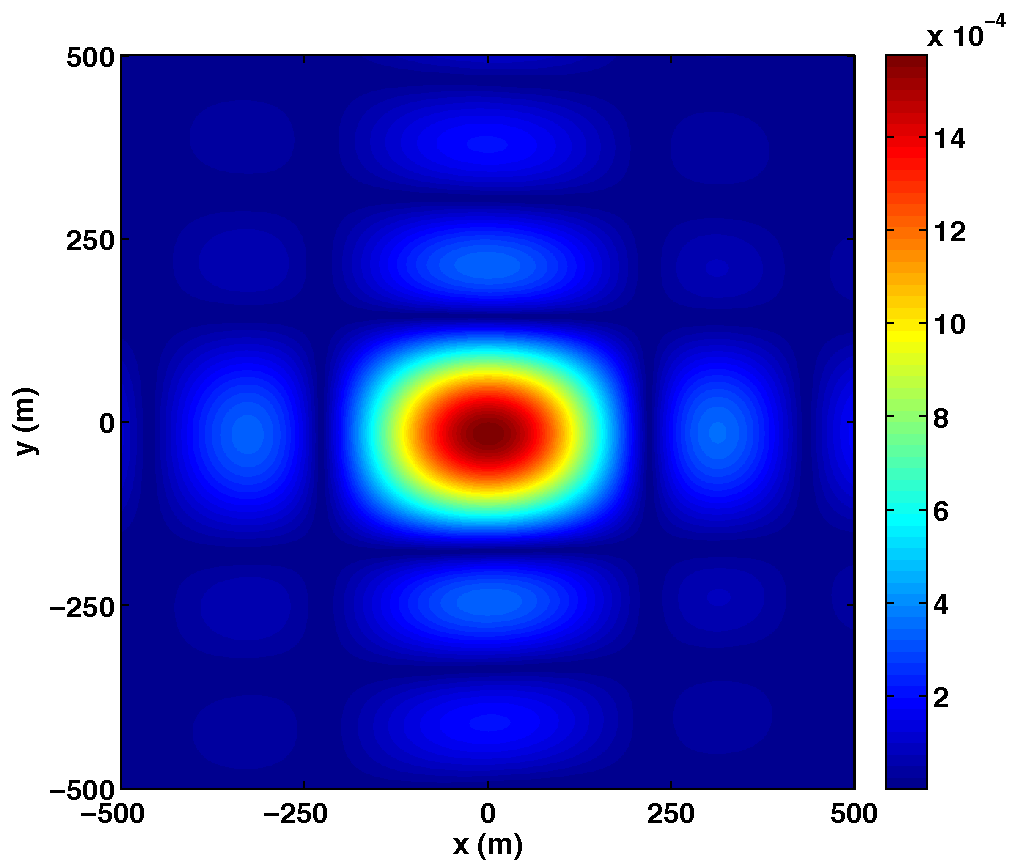
\includegraphics[scale=0.5]{figures/beamfootprint}
  \caption[Colorful Picture]{This is a colorful picture.}%
  \label{fig:flyover}
\end{figure}
\end{comment}


\begin{comment}
\begin{table}[p]
  \centering
\begin{tabular}{llr}
\toprule
\multicolumn{2}{c}{Item} \\
\cmidrule(r){1-2}
Animal    & Description & Price (\$) \\
\midrule
Gnat      & per gram    & 13.65      \\
          & each        & 0.01       \\
Gnu       & stuffed     & 92.50      \\
Emu       & stuffed     & 33.33      \\
Armadillo & frozen      & 8.99       \\
\bottomrule
\end{tabular}
  \caption[Table Example]{This table shows some data}%
  \label{tab:myfirsttable}
\end{table}
\end{comment}
